La \emph{Computer Vision} (ou vision par ordinateur) comprend l'acquisition, l'analyse et
le traitement des images numériques pour comprendre et extraire des données, informations
ou décisions.\\
Les applications et possibilités de ce domaine sont pour ainsi dire, infinie.

\section{Défis liés à la mesure en extérieur}
La principale difficulté de la mesure de neige par \emph{Computer Vision} est lié au fait
qu'il neige. Les caméras embarquées sont souvent de mauvaise qualité, et les débits
sont mauvais à cause des processeurs embarqués qui sont limités en puissance de calcul.

\begin{figure}[H]
    \centering
    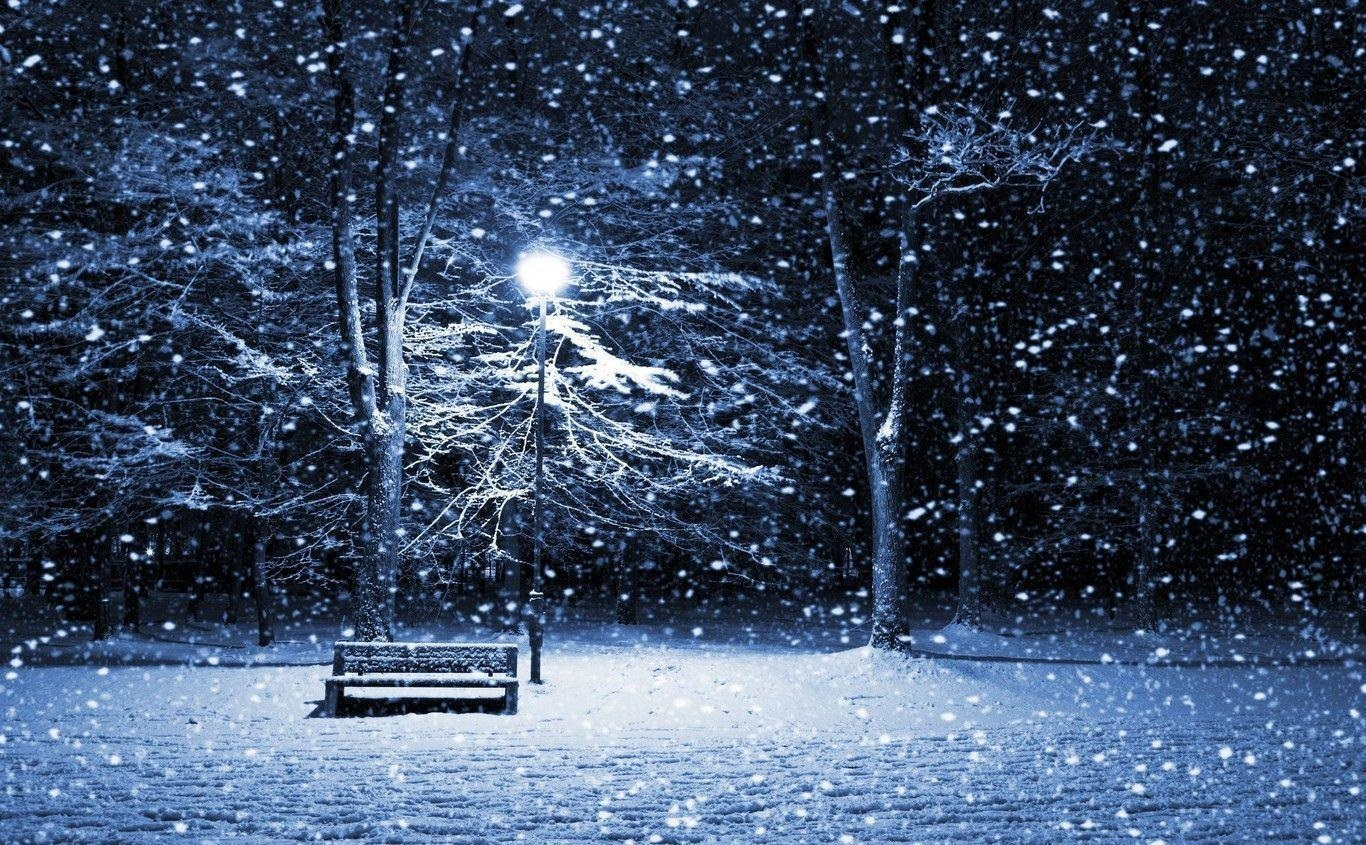
\includegraphics[width=0.4\textwidth]{Images/computer_vision/perfect_snow.jpg}
    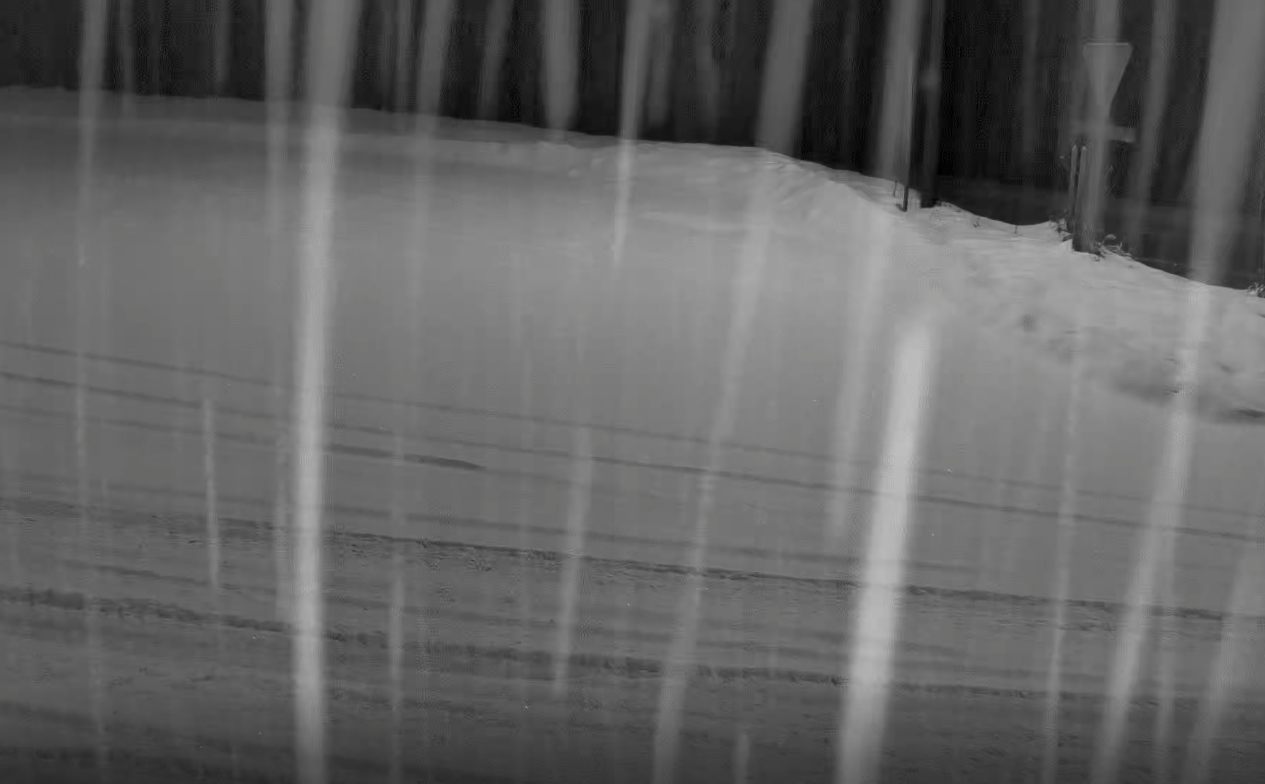
\includegraphics[width=0.4\textwidth]{Images/computer_vision/real_snow.png}
    \caption[Comparaison image de neige HD et cas concret]{Comparaison entre une image idéale \footnotemark[1] et un cas concret\footnotemark[2]}
    \label{fig:Snow comparison}
\end{figure}
\footnotetext[1]{Wallpaper from WallpaperCave, by caveman, \url{https://wallpapercave.com/w/scDoVwf} (last accessed: 20 January 2022)}
\footnotetext[2]{VibroSnow camera, implemented at route du Pralan, Ayent, Suisse}

\noindent
Il faut donc trouver une méthode ne demandant pas trop de ressources de calcul, et pouvant fournir
des résultats utiles pour informer sur l'état des routes.

\section{Applications pour la mesure de neige}
Les possibilités de la \emph{Computer Vision} étant vaste, plusieurs méthodes ont été discutées.

\newpage

\subsection{Mesure de niveau sur une règlette}
Les mesures de niveau de neige manuel se font déjà avec une réglette plantée dans la neige.

\begin{figure}[H]
    \centering
    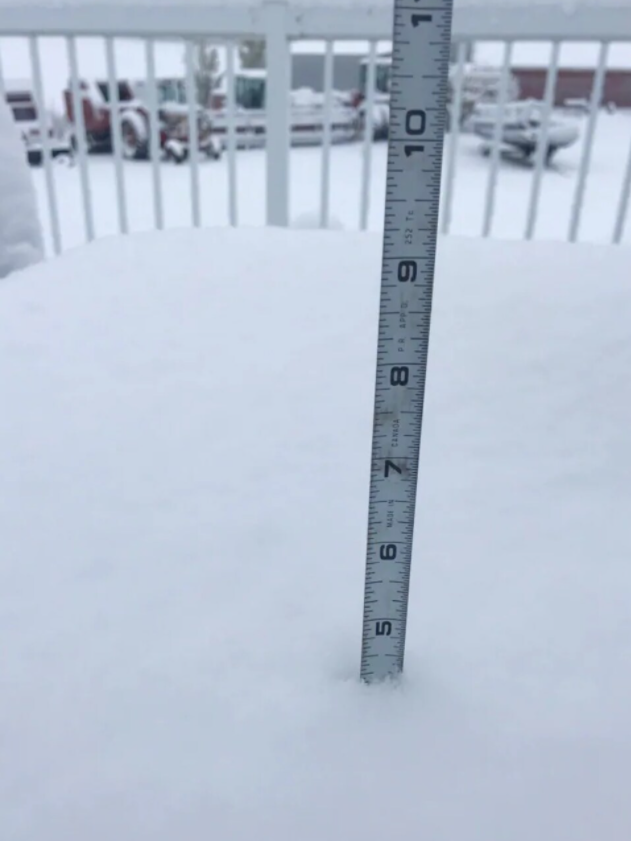
\includegraphics[width=0.3\textwidth]{Images/computer_vision/snow_meter.PNG}
    \caption[Mesure de neige à la règle]{Mesure d'environ 4.5 pouces de neige à Manitoba, Canada\footnotemark[1]}
    \label{fig:Snow meter}
\end{figure}
\footnotetext[1]{Image by Jerry Zachedniak, \url{https://ici.radio-canada.ca/nouvelle/1338531/hiver-tempete-parc-mont-riding}
(last accessed: 20 January 2022)}
\noindent
La mesure pourrait être réalisé en plaçant la caméra en face de la règlette.
Deux méthodes sont possibles :
\begin{description}
    \item[Avoir une règlette graduée] \hfill \\
    et compter le nombre de graduation encore visible pour déterminer la hauteur de neige.
    \item[Avoir un piquet d'une taille connue] \hfill \\
    comparer la hauteur de ce piquet au nombre de pixel quand il n'y a pas de neige,
    puis mesurer le nombre de pixels non-ensevelis pour mesurer la hauteur de neige.
\end{description}
\noindent
Cependant mesurer une règlette peut paraître simple d'un point de vue de l'implémentation,
mais présente plusieurs désavantages lors du fonctionnement:

\begin{description}
    \item[Il faut déneiger devant la caméra et la règlette] \hfill \\
    demandant probablement à un ouvrier de descendre de son chasse-neige pour déneiger l'installation.
    \item[L'installation ne doit pas être trop proche d'une route] \hfill \\ 
    de risque d'être ensevelie ou endommagée lors du passage d'un chasse-neige.
    \item[Si on utilise une règlette graduée] \hfill \\ 
    il faut s'assurer d'avoir un matériau surlequel la neige ne colle pas ou 
    ne réfléchis pas trop la lumière du soleil.
    \item[L'utilisation d'un piquet peut demander l'usage d'une intelligence artificielle] \hfill \\
    pour reconnaitre le piquet d'autres objets (p. ex.: arbres, lampadaires, ...) \cite{SnowTimeLapse}%\footnotemark[2])
    Cela demanderait trop de puissance de calcul pour un système embarqué basse consommation.
    Une autre solution serait de calibrer chaque installation pour reconnaître le piquet.
    Cependant la caméra étant intégrée dans un système embarqué, cette calibration serait certainement
    fastidieuse et demanderait une interface utilisateur supplémentaire pour la réaliser.
\end{description}
%\footnotetext[2]{\emph{Snow Depth Measurement via Time Lapse Photography and Automated Image Recognition},
%by Kevin S. J. Brown and Steven R. Fassnacht at Colorado State University,
%Departement of Ecosystem Science and Sustainability, 2019, http://www.codos.org/\#lit}
\newpage

\subsection{Mesure de niveau par Stéréovision}
La Stéréovision est une méthode de mesure se servant d'images provenant de plusieurs point de vue.
Typiquement, deux caméras côte à côte, peuvent mesurer des profondeurs comme des yeux.

\begin{figure}[H]
    \centering
    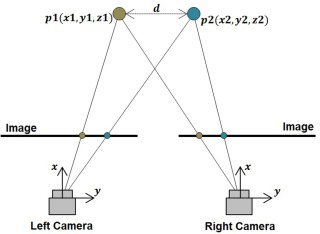
\includegraphics[width=0.5\textwidth]{Images/computer_vision/stereovision.jpg}
    \caption[Schéma de principe stéréovision]{Schéma de principe de mesure de distance par stéréovision}
    \label{fig:Stereovision}
\end{figure}
\noindent
Beaucoup de caméra spécialisée dans la reconnaissance d'image par Intelligence artificielle utilise se principe
pour estimer les distances (ex: OpenCV OAK cameras).
Cette méthode demande trop de puissance de calcul pour un système embarqué basse consommation et ne fournit
pas de résultat suffisamment précis pour mesurer une couche de neige.
\newpage

\subsection{Mesure du débit de chute de neige}
Une mesure simple et rapide est d'estimer le débit de chute de neige en isolant les flocons.
\begin{figure}[H]
    \centering
    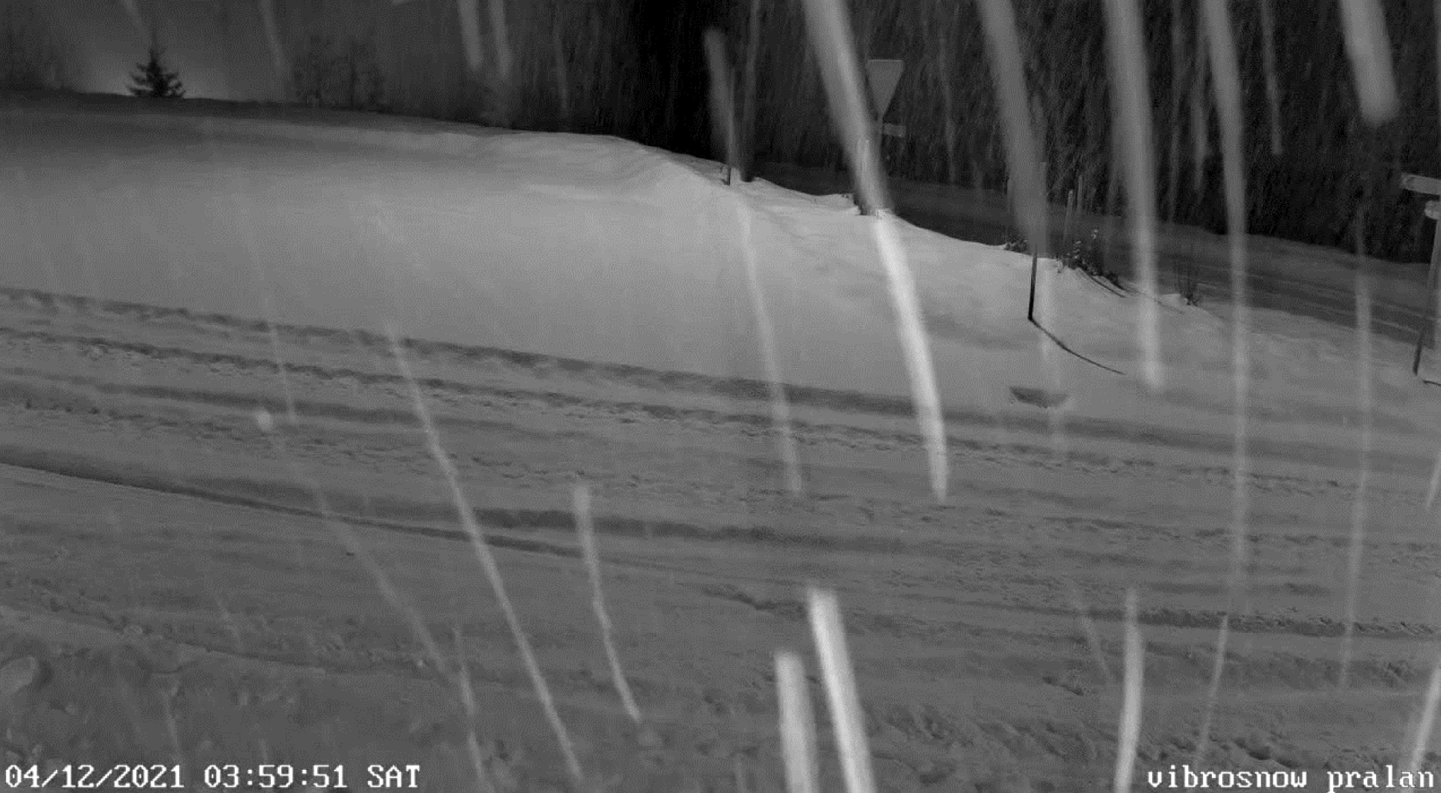
\includegraphics[width=0.35\textwidth]{Images/computer_vision/snow_cam.png}
    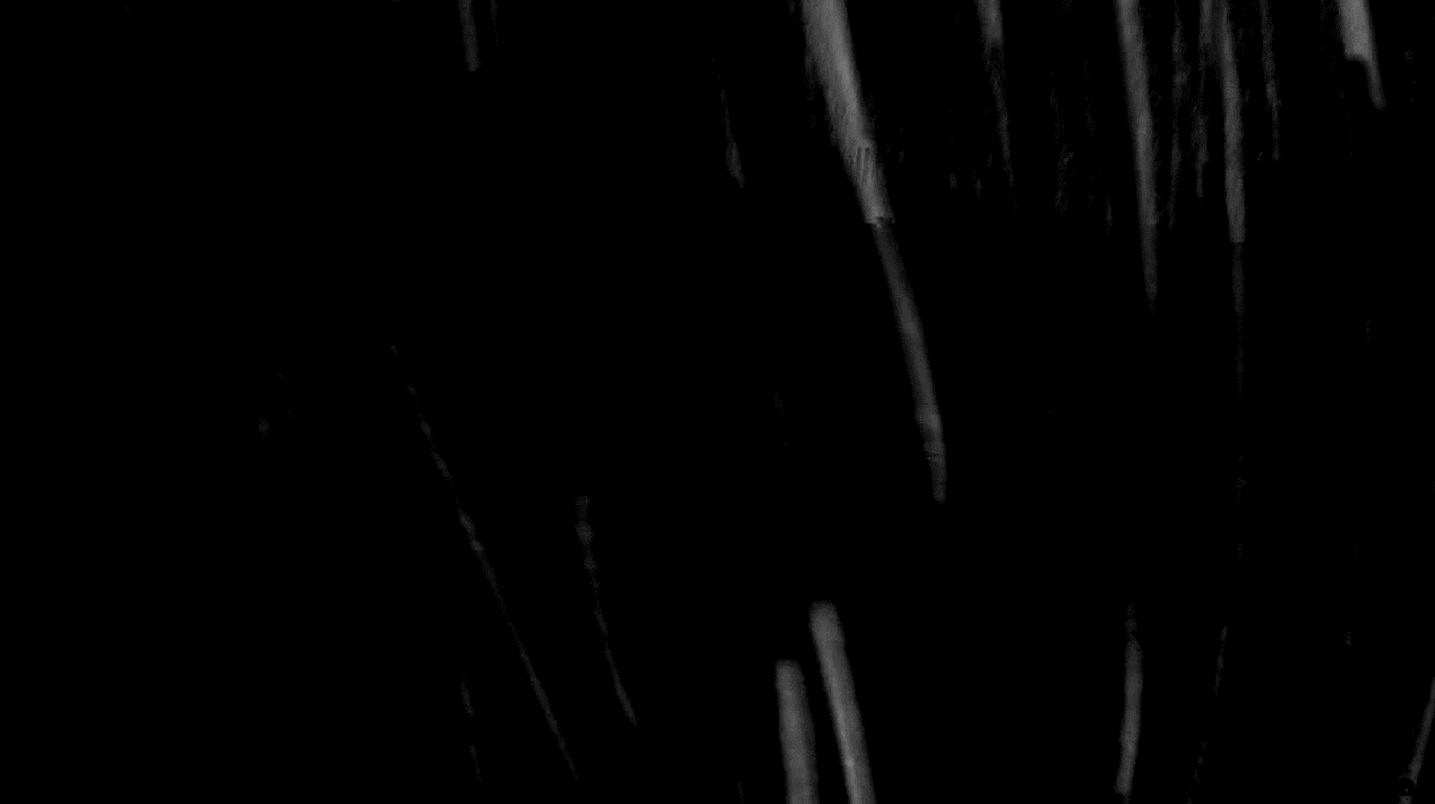
\includegraphics[width=0.35\textwidth]{Images/computer_vision/snowfall.png}
    \caption[Comparaison image source et bruit sur image]{Image source de la caméra VibroSnow\footnotemark[1] et image avec les flocons isolés}
    \label{fig:Snowfall}
\end{figure}
\footnotetext[1]{VibroSnow camera, implemented at route du Pralan, Ayent, Suisse}
\noindent
Cette mesure, en parrallèle à une mesure de hauteur de neige, permettrait d'estimer 
l'augmentation de cette hauteur au fil du temps. Fournissant ainsi une information supplémentaire
aux services de déneigement.

\subsection{Détection de route enneigée}
Étant donné que la mesure de hauteur de neige par \emph{Computer Vision} serait trop complexe
pour un système embarqué basse consommation, détecter si la route est enneigée ou non
permettrait de fournir une redondance à une mesure de hauteur de neige fournie par un autre capteur.
Si la petite zone mesurée par le capteur se retrouve mal déneigée, ou qu'un objet, comme un caillou, mal placé
fausse la mesure du capteur, savoir si le segment de route est enneigé ou non permettrait d'éliminer ces erreurs.

\subsection{Méthodes retenues}
Les méthodes retenues pour ce projet de recherche sont \textbf{la mesure du débit de chute de neige}
et \textbf{la détection de route enneigée}. Elles peuvent fournir des informations pertinentes
pour le déneigement, tout en demandant relativement peu de puissance de calcul.
\newpage